\chapter{Arquitetura Básica do RouteFlow}

\section{Introdução ao Projeto Comunitário RouteFlow}

O projeto comunitário RouteFlow é uma proposta de oferta de serviços de
roteamento IP remoto de forma centralizada, e que visa um
desacoplamento efetivo entre o plano de encaminhamento e o
plano de controle (ROUTEFLOW, 2011). O objetivo é tornar as
redes IP mais flexíveis pela facilidade de adição,
remoção e especialização de protocolos e algoritmos.


O RouteFlow prove um serviço virtualizado de roteamento IP
em equipamentos com suporte ao protocolo \textit{OpenFlow}
seguindo o paradigma das redes definidas por software.
Basicamente, o RouteFlow interliga uma infraestrutura 
\textit{OpenFlow} com um ambiente virtual de roteamento 
IP baseado em ferramentas nativas do Linux (Quagga) para
um roteamento eficiente na estrutura física. Baseado em um
sistema de controle RouteFlow, os \textit{switches} 
são instruídos via controladores \textit{OpenFlow} que 
trabalham como proxies no intuito de traduzir as mensagens
e eventos entre o ambiente físico e virtual. 

O projeto conta com um número crescente de usuários no 
mundo (cerca de 1000 downloads e mais de 10000 visitantes
desde que o projeto começou em Abril de 2010). As principais
formas de contribuição para o projeto é através do sistema
de repositórios GitHub. Para citar alguns exemplos de contribuição
por parte da comunidade, é possível citar a contribuição
do Google nos plugins SNMP e o trabalho atual no suporte
ao MPLS e nas APIs de roteamento Quagga. A universidade
americana de Indiana contribuiu com uma interface gráfica
e com a execução de um piloto em seu \textit{testbed}.
% É possível adicionar mais exemplos de contribuições externas


O RouteFlow é composto basicamente por três módulos principais:
o cliente RouteFlow (RFClient), o servidor RouteFlow (RFServer) e
o proxy RouteFlow. Todos os módulos serão
explicados com mais detalhes nas seções seguintes. A Figura \ref{fig:visaoGeralRouteFlow} mostra
de forma simplificada um cenário RouteFlow típico: engines de 
roteamento em um ambiente virtual geram uma base de 
informação de encaminhamento baseado nos protocolos 
de roteamento (OSPF, BGP) e processos ARP. Durante a 
execução do ambiente virtual, as tabelas de roteamento e 
tabelas ARP são coletadas pelos módulos clientes (RFClient) executando
nas máquinas virtuais e traduzido em tuplas OpenFlow que
são enviadas para o servidor (RFServer), que faz a adaptação das 
informações para o ambiente físico e finalmente instrui o 
módulo proxy (RFProxy), uma aplicação controladora, para configurar
os \textit{switches OpenFlow} no ambiente físico.


\begin{figure}[h]
\centering
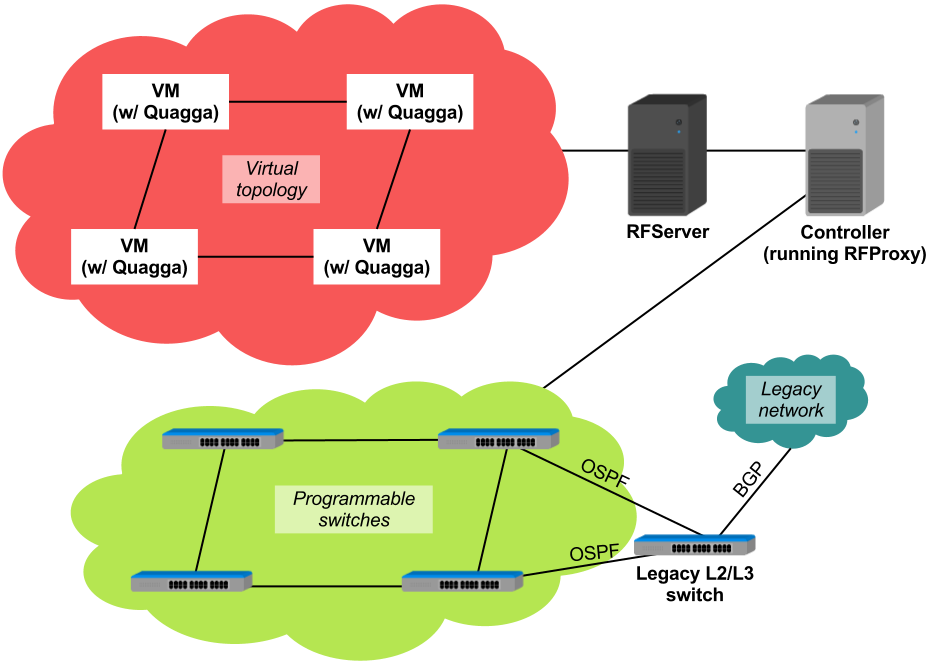
\includegraphics[width=160mm]{visaoGeralRouteFlow.png}
\caption{Visão geral do RouteFlow.}
\label{fig:visaoGeralRouteFlow} 
\end{figure}


Pacotes de encaminhamento dos protocolos de roteamento 
e controle de tráfico (ARP, BGP, RIP e OSPF) são direcionados
pelo proxy (RFProxy) para as interfaces virtuais correspondentes do
ambiente virtual. Entre o ambiente virtual e o ambiente existe
um switch virtual que também é controlado pelo proxy (RFProxy),
permitindo um caminho direto entre os ambientes, reduzindo 
o tempo das trocas de mensagens e sem a necessidade de passar
através do servidor (RFServer) e do cliente (RFClient).

Abaixo temos os principais avanços da arquitetura do projeto
RouteFlow

\begin{itemize}
\item \textbf{Plataforma totalmente modular, extensível, 
configurável e flexível.} A arquitetura atual do RouteFlow 
foi feita pensando em sua própria evolução. Através do 
conceito de camadas, o RouteFlow conseguiu facilitar o entendimento
geral do código, facilitando o seu entendimento total por parte de 
seus usuários. A construção baseada em módulos independentes
torna o código mais claro, facilitando a portabilidade para outras 
linguagens ou o suporte à novas tecnologias. O exemplo mais 
claro sobre a independência dos módulos é o próprio módulo levado em consideração
na construção do trabalho de conclusão de curso em questão, o
proxy (RFProxy). 

O proxy (RFProxy) faz a troca de mensagens com os outros módulos 
através de um sistema de banco de dados, sendo facilmente
portado para outras linguagens de programação e tecnologias.

Outro beneficio da construção baseada em módulos é a possibilidade
de execução do RouteFlow em múltiplos sistemas computacionais, 
fazendo-o executar como uma arquitetura distribuída. Tal 
característica será melhor explica nos itens abaixo.
\item \textbf{Suporte à replicação do estado da rede e grande
disponibilidade dos recursos.} Para melhorar a disponibilidade
do sistema, o RouteFlow foi construído de forma descentralizada, 
separando os dados relacionados ao estado das redes dos módulos de processamento.
Todos os dados relacionados ao estado das redes é armazenado
em um banco de dados centralizado, possibilitando que qualquer aplicação 
registrada tenha acesso. Dessa maneira é possível obter uma 
replicação dos processos, obtendo as vantagens e benefícios
de um sistema descentralizado. 

A versão atual do projeto ainda
não faz duplicação dos processos mas a ideia já é levada em
consideração para futuras implementações. 
\item \textbf{Armazenamento do histórico da rede e de estatísticas.}
Como citado no item anterior, a ideia de descentralização do RouteFlow
fez que os dados fossem armazenados em um banco de 
dados centralizado. Esse características traz consigo
uma série de vantagens, além de todas citadas anteriormente, ainda pode ser 
mencionado a possibilidade
de se manter um histórico das ações e decisões tomadas pelo
sistema. O RouteFlow, através do banco de dados centralizado, mantem 
um histórico de todo o sistema, bem como as estatísticas relacionadas 
à criação de regras e ao uso da rede. Tais características permitem
 aos pesquisadores
ou até mesmo aos administradores de redes ter um controle 
e um entendimento mais elaborado, podendo reproduzir o ambiente
em certos períodos de tempo. Sendo possível reproduzir o sistema
em ambientes em que o mesmo apresentou certa irregularidade ou
falha. 
As estatística ainda dão ao administrador um entendimento maior 
de como a rede é usada, possibilitando ao mesmo a tomada de
alguma decisão para a busca de melhorias.
\item \textbf{Possibilidade de ambientes com múltiplos controladores
\textit{OpenFlow}.} A arquitetura atual do RouteFlow foi
desenvolvida para ter suporte em cenários com múltiplos controladores
\textit{OpenFlow}. Tal característica permite aos pesquisadores
ou administradores particionar a rede e controlar cada região
com um controlador independente. Outro fator interessante é
que as camadas superiores do RouteFlow abstraem as diferenças
entre as versões 1.0/1.1/1.2/1.2 do OpenFlow, tornando fácil o
suporte à controladores heterogêneos. 
Para que tal característica fosse suportada, o código do RouteFlow
passou por um processo de padronização, melhorando ainda 
mais a legibilidade do projeto.
\end{itemize}

% Melhorar o titulo
\section{Banco de Dados Centralizado com Suporte a IPC}

Nesse capitulo será explicado com detalhes a arquitetura de 
banco de dados centralizado e seu suporte aos mecanismos
de comunicação entre processos usados pelo projeto RouteFlow.
Também serão abordados as principais vantagens e desvantagens
da arquitetura.

Várias abordagens foram proposta pelo RouteFlow para um
esquema unificado de comunicação entre processos (IPC). 
Inúmeras delas foram testadas e avaliadas até se conseguir 
traçar as principais vantagens e desvantagens de cada uma delas.
Soluções baseadas em filas de mensagens, como o RabbitMQ
ou o ZeroMQ foram descartadas por causa da grande complexidade
de implementação e manutenção. Soluções baseadas em serialização
de mensagens, como ProtoBuffers e Thrift, se apresentaram como
boas soluções mas requiriam uma lógica adicional para o armazenamento
pendente e para mensagens já consumidas. Durante o estudo
de banco de dados Não SQL para armazenamento persistente,
surgiu as primeiras ideias do uso de um banco de dados como
ponto central de um mecanismo de troca de mensagens entre 
processos (IPC) e consequentemente manter o histórico das 
ações tomadas pelo RouteFlow para permitir a replicação de certas
situações.

Depois de levar em consideração as mais populares opções de 
banco de dados Não SQL (MongoDB, Redis, CouchDB), foi 
decidido sobre a implementação de um banco de dados centralizado
e dos mecanismos de troca de mensagens entre processos (IPC) 
utilizando-se o MongoDB. Os principais fatores para a escolha foram
a facilidade de programação, suporte nativo a inúmeras linguagens de 
programação, suporte nativo à tecnologia JSON e a existência de 
mecanismo para replicação e distribuição. A ideia por trás do
mecanismo de troca de mensagens (IPC) é completamente
independente da escolha do banco de dados e por isso não 
foi levada em consideração.

No núcleo do RouteFlow estão os mapeamentos entre o ambiente
físico controlado e o ambiente virtual executando as tarefas de
roteamento. A confiabilidade desses estados de rede é imprescindível 
para o servidor (RFServer) e se torna difícil de manter sem a ajuda de 
algum módulo externo. Um banco de dados externo se encarrega
desse objetivo, tendo sua configuração mais flexível. Estatísticas
coletadas pelo proxy (RFProxy) também podem ser armazenadas em 
um banco de dados centralizado, baseado em serviços adicionais
é até possível implementar ferramentas para análise dos dados 
ou até mesmo visualização.

A escolha de delegar o controle dos estados da rede para um
banco de dados permite uma melhor tolerância a falhas, replicando
a base de dados ou até mesmo separando o servidor (RFServer) em várias
instâncias. A possibilidade de distribuição do servidor (RFServer) permite
ao sistema um melhor desempenho, sendo possível distribuí-lo
em vários pontos de uma rede e assim reduzindo a latência de
comunicação. Já é levado em consideração o uso de um banco de
dados distribuído para as próximas atualizações do RouteFlow.

A implementação atual do RouteFlow leva em consideração
as melhores técnicas e práticas usadas em aplicações executando
nas nuvens, isso inclui recursos de escalabilidade, banco de 
dados tolerante à falhas que serve como mecanismo de troca
de mensagens entre processos (IPC), controle centralizado
do estado da rede, armazenamento das informações usadas 
para desenvolvimento de aplicações de roteamento (histograma 
de tráfico, monitoramento de fluxos e ações administrativas).
Assim podemos dizer que o banco de dados nos provê uma 
base com informações da rede (\textit{Network Information
Base, NIB}) [Koponen et al. 2010] e uma base de conhecimento
 (\textit{Knowledge Information Base, KIB}) [Saucez et al. 2011].

\section{Esquema de Configuração Flexível}

Nas primeiras versões do RouteFlow, a associação entre máquinas
virtuais (executando o cliente RouteFlow) e os \textit{switches OpenFlow}
era feita de forma automática e gerenciada pelo servidor (RFServer) baseado
no critério de ordem de registração: o cliente de numero um
era associado ao primeiro switch à ingressar na rede, o de número
dois ao segundo e assim diante. Essa característica não requeria 
que o administrador controla-se o registro dos switches na rede mas
era necessário tomar conta da ordem de ingresso dos switches.

Essa abordagem funcionou bem em ambientes controlados e 
experimentais mas apresentou problemas em ambientes onde
os switches não eram controlados diretamente pelo administrador.
Para resolver este problema e ser base para o suporte ao uso de
múltiplos controladores, a implementação atual do RouteFlow
faz uso de um mapeamento 1:1 definido de forma manual pelo 
administrador da rede.
É necessário o conhecimento prévio da rede pelo administrador
para que o mapeamento seja feito de forma correta. Esse mapeamento
é carregado e armazenado no banco de dados centralizado.
A Tabela \ref{tab:tipos_associacao} demonstra os possíveis estados que o mapeamento
pode assumir. A Figura \ref{fig:rfserverAssociacao} ilustra como o RFServer trata os eventos
da rede.


\begin{table}[h]
\centering
\begin{tabular}{|l|c|c|}
\hline
Formato & Tipo\\
\hline
\hline
$vm_-id,vm_-port,-,-,-,-,-$ & Porta do Cliente Inativa\\
\hline
$-,-,-,-,-,dp_-id,dp_-port,ct_-id$ & Porta do Switch Inativa\\
\hline
$vm_-id,vm_-port,dp_-id,dp_-port,-,-,ct_-id$ & Associação entre Cliente e Switch\\
\hline
$vm_-id,vm_-port,dp_-id,dp_-port,vs_-id,vs_-port,ct_-id$ & Associação entre Cliente e Switch Ativa\\
\hline
\end{tabular}
\caption{Tipos possíveis de associação}
\label{tab:tipos_associacao}
\end{table}


Sempre que um switch OpenFlow ingressa na rede, o proxy (RFProxy)
informa ao servidor RouteFlow (RFServer) sobre cada uma das
portas físicas. Cada uma dessas portas é registrada pelo servidor
em um dos dois tipos mostrados na Tabela \ref{tab:tipos_associacao}:
como (i) \textit{Porta de Switch Inativa} ou (ii) \textit{Associação
entre Cliente e Switch}. Essa associação ocorre quanto 
não há nenhuma configuração para a porta do switch que
foi registrada ou a porta cliente configurada para ser associada
com essa porta do switch ainda não foi registrada. A última 
opção acontece quando a porta do cliente a ser associada com a
porta do switch (baseada na configuração prévia do ambiente)
está pronta e registrada como inativa.

Quando um cliente (RFClient) inicia, o mesmo informa ao servidor RouteFlow (RFServer)
informações sobre suas interfaces (portas). Essas portas são 
registradas pelo RFServer em um dos estados mostrados na
Tabela \ref{tab:tipos_associacao}: como uma porta de cliente
inativa ou como uma associação entre cliente e switch. A 
associação é análoga a associação descrita às portas dos
switches.

Depois da associação, o servidor (RFServer) solicita ao cliente (RFClient) para
disparar a mensagem que irá confirmar que o switch virtual está
conectado e apto a se comunicar com o proxy (RFProxy). Quando isso
acontece, o proxy (RFProxy) é alertado sobre a conexão entre o 
cliente (RFClient) e seu switch virtual, e envia uma informação ao 
servidor (RFServer). O servidor (RFServer) decide o que fazer com a informação.
Tipicamente, o proxy (RFProxy) é intruido a redirecionar todo o tráfego
das máquinas virtuais para os switches físicos associados e 
vice-versa. Quando um switch abandona a rede, todas as 
associações envolvendo as portas do mesmo são removidas,
deixando inativas as portas do cliente envolvidas na associação.
Em caso de conexão de um switch, o RouteFlow checa se o 
mesmo é um novo ingressante ou se é um retornante, podendo
apenas restaurar as associações configuradas previamente 
pelo administrador.


\begin{figure}[h]
\centering
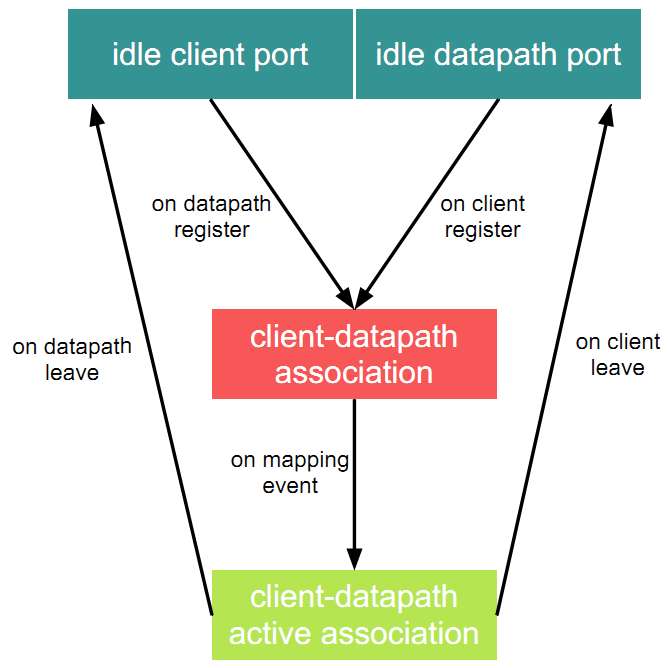
\includegraphics[width=120mm]{rfserverAssociacao.png}
\caption{Tratamento de Associações do RFServer.}
\label{fig:rfserverAssociacao} 
\end{figure}


Uma entrada no arquivo de configuração contem um conjunto 
dos campos identificados na Tabela \ref{tab:tipos_associacao}:
\textit{$vm_-id, vm_-port, dp_-id, dp_-port, ct_-id$}. Esses campos
são suficientes para a associação, os campos remanescentes
são relacionados à conexão com o switch virtual ($vs_-*$) e serão
definidos em tempo de execução. O campo \textit{$ct_-id$} identifica
identifica com qual controlador o switch está conectado. Esse
mecanismo permite ao RouteFlow trabalhar com múltiplos
controladores, cada um controlando uma parte da mesma rede.

Considerando que o ambiente virtual pode ser distribuído, é 
possível executar vários domínios de roteamento com um
único servidor (RFServer), facilitando o gerenciamento de inúmeras 
redes roteadas em um único ponto.

\section{Descrições dos Principais Módulos do RouteFlow}
Como citado nas seções acima, O RouteFlow é dividido em 
três módulos básicos: cliente (RFClient), servidor (RFServer)
 e proxy (RFProxy). Na Figura
\ref{fig:componentesRouteFlow} temos uma visão geral das
aplicações:


\begin{figure}[h] 
\centering
\includegraphics[width=130mm]{componentesRouteFlow.png}
\caption{Componentes principais do RouteFlow.}
\label{fig:componentesRouteFlow} 
\end{figure}


\begin{itemize} 
\item RFClient executa como um programa
executável em um máquina virtual, detectando
mudanças na tabela ARP do Linux e na tabela de roteamento.
As informações sobre rotas são enviadas para o
servidor (RFServer) quando são atualizadas pelas aplicações
encarregadas do roteamento (QUAGGA). 

\item RFServer é uma aplicação independente que gerencia as
máquinas virtuais que estão executando o cliente (RFClient). 

O RFServer mantem o mapeamento entre as instâncias das
máquinas virtuais executando o cliente (RFClient) e as interfaces
correspondentes aos \textit{switches} e suas respectivas portas. É
conectado ao proxy (RFProxy) para instruí-lo como configurar os
fluxos e também como configurar o Open vSwitch que mantém a
conectividade de todo o ambiente composto pelas máquinas virtuais.
É considerado o módulo mais importante e mais complexo
do projeto RouteFlow.

\item RFProxy é uma aplicação responsável pelas interações
entre os switches \textit{OpenFlow} (identificados pelos seus
datapaths) via o protocolo \textit{OpenFlow} e os demais
módulos do ambiente, como o servidor (RFServer) e o conjunto
de clientes (RFClients). Ele aguarda instruções
do servidor (RFServer) e o notifica à respeito de todos os eventos da rede.
Atualmente é executado como um módulo vinculado aos
controladores \textit{OpenFlow}. 

O RouteFlow tem suporte aos
controladores NOX e POX, sendo que a proposta do trabalho é
adicionar suporte ao controlador Floodlight. 
\end{itemize}

\section{Protocolo RouteFlow}

É o protocolo desenvolvido e usado para a comunicação entre
os componentes do RouteFlow. Nele, estão definidas as
mensagens e os comandos básicos para conexão e configuração
das máquinas virtuais e, também, gerenciamento das entradas
de roteamento em hardware. Entre os campos da
mensagem-padrão estão: identificação do controlador,
identificação da máquina virtual, tipo da mensagem,
comprimento e dados. 

O proxy (RFProxy) recebe os comandos do
servidor (RFServer) através deste protocolo e de acordo com o
tipo de comando executa as principais ações, muitas delas
exigindo a comunicação com os switches físicos. A
comunicação com os switches físicos é feita via protocolo
\textit{OpenFlow}, fazendo o proxy RouteFlow agir como
uma espécie de "tradutor" entre os dois protocolos.
